\subsubsection{Latent heat benchmark}
\label{sec:benchmark-latent_heat}

\textit{This section was contributed by Juliane Dannberg.}

The setup of this benchmark is taken from Schubert, Turcotte and Olson \cite{STO01} (part 1, p. 194) and is illustrated in Fig.~\ref{fig:latent-heat-benchmark}.
\begin{figure}
  \begin{center}
    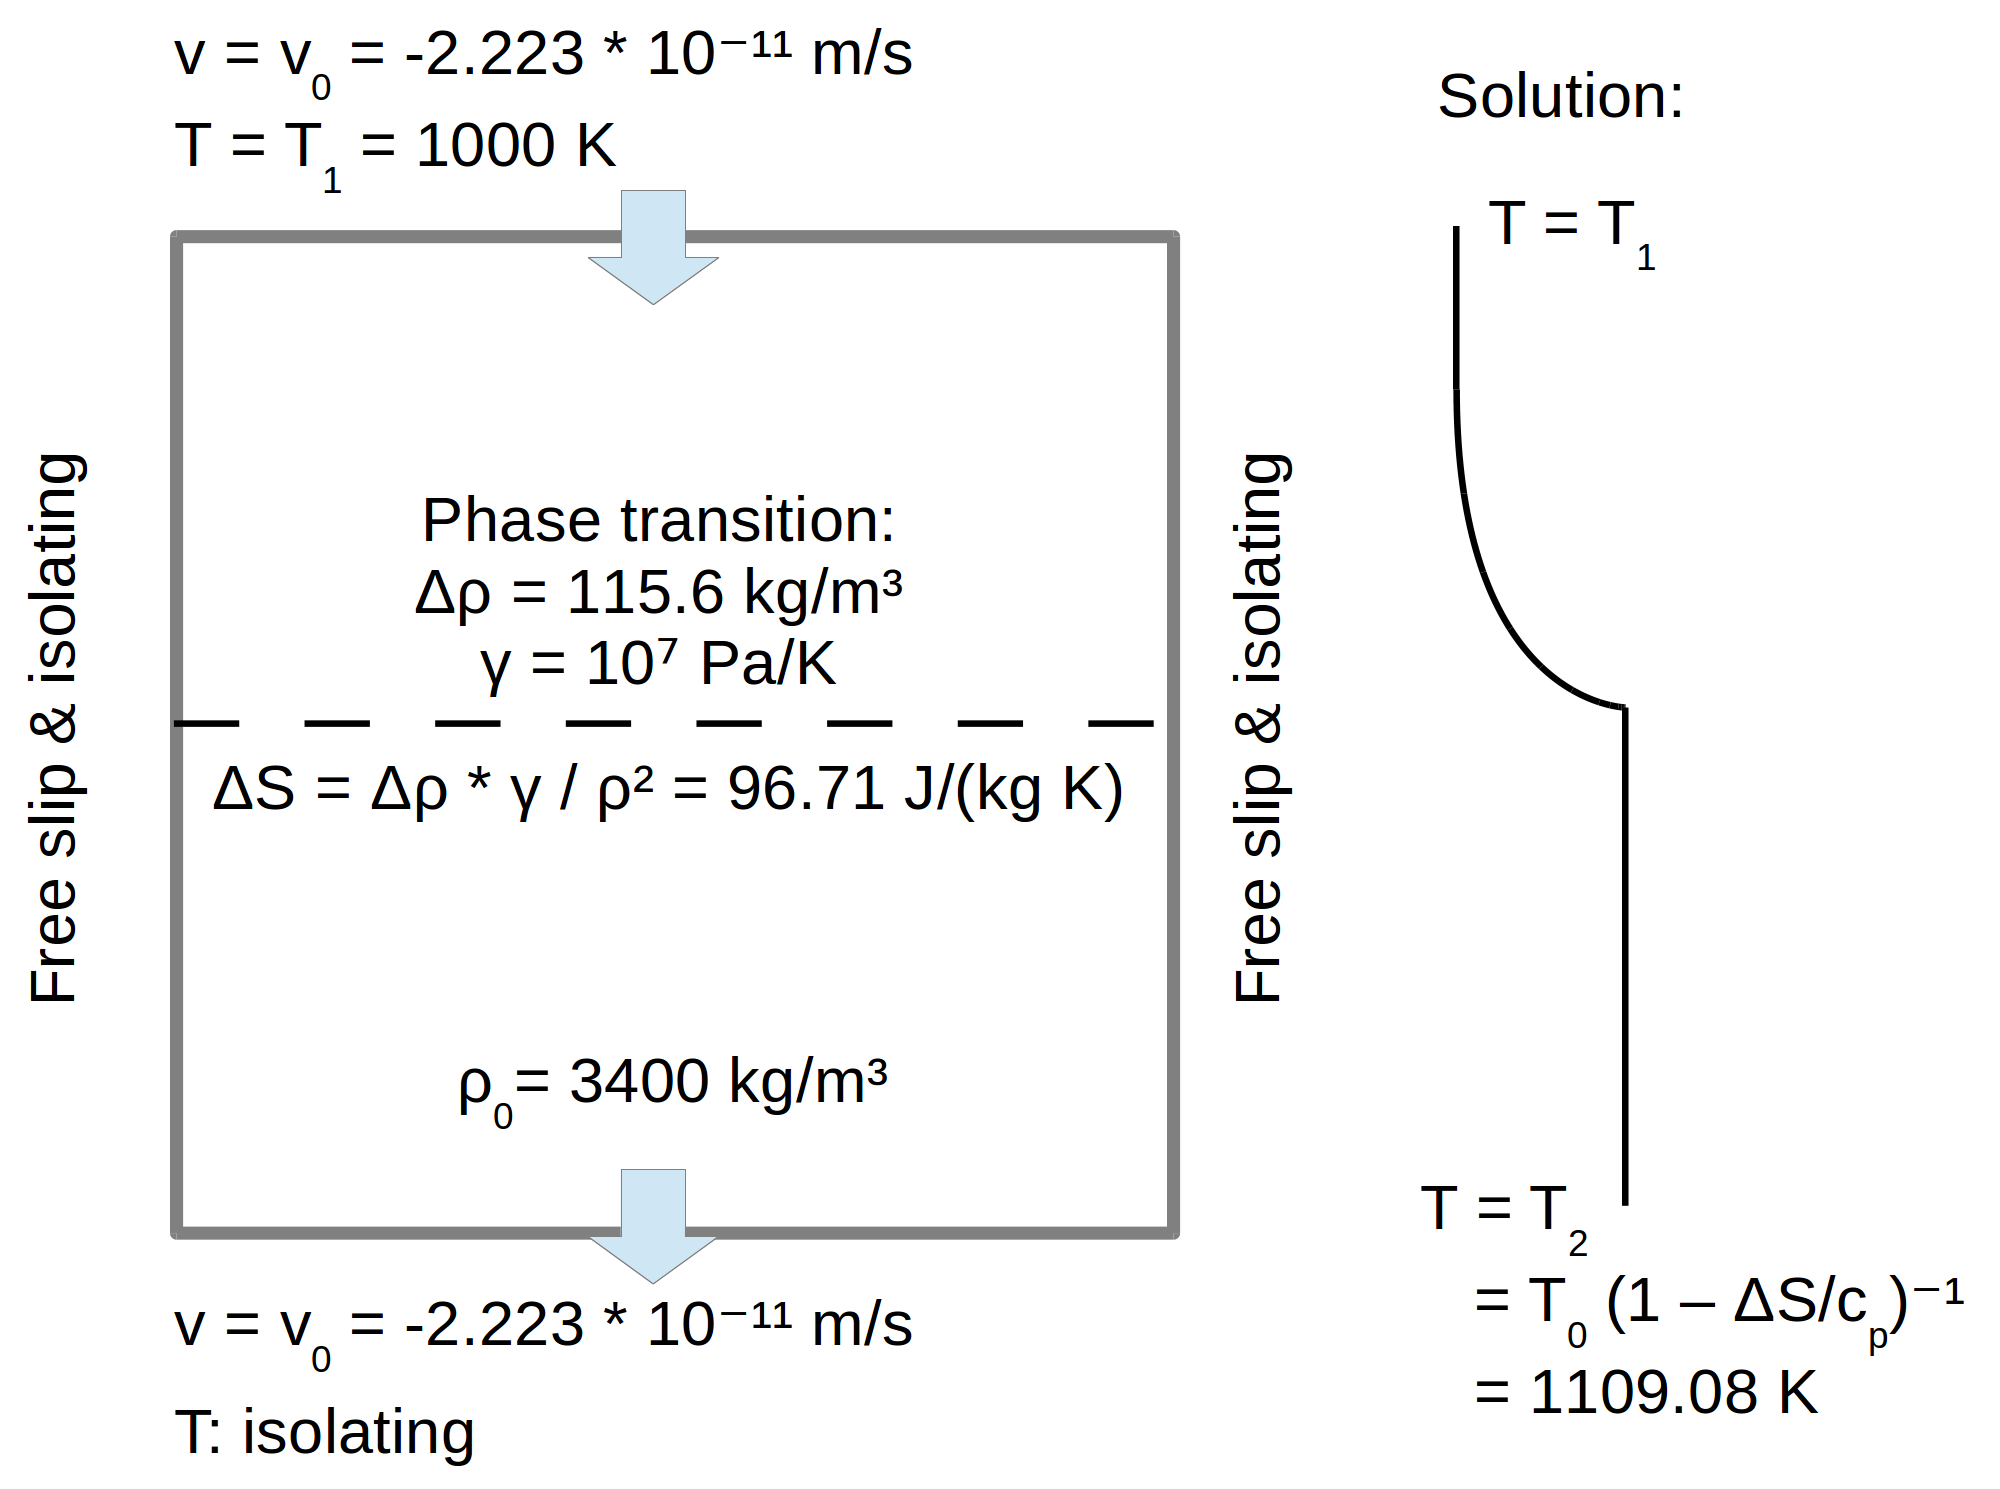
\includegraphics[width=0.52\textwidth]{cookbooks/benchmarks/latent-heat/doc/latent-heat-setup.png}
    \hfill
    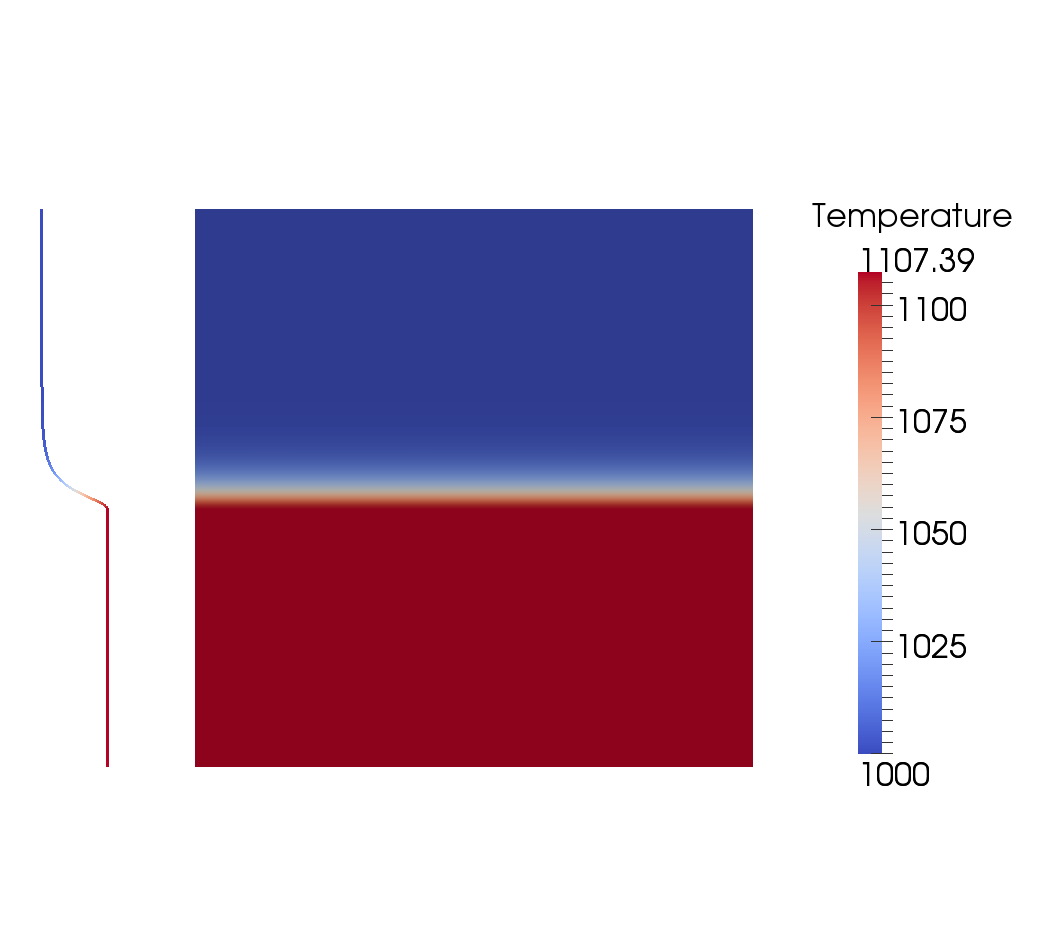
\includegraphics[width=0.47\textwidth]{cookbooks/benchmarks/latent-heat/doc/latent-heat-temperature.png}
  \end{center}
  \caption{\it Latent heat benchmark. Both figures show the 2D box model domain.
      Left: Setup of the benchmark together with a sketch of the expected
      temperature profile across the phase transition. The dashed line marks
      the phase transition. Material flows in with a prescribed temperature and
      velocity at the top, crosses the phase transition in the center and flows
      out at the bottom. The predicted bottom temperature is $T_2 = 1109.08 \, \si{K}$.
      Right: Temperature distribution of the model together with the associated
      temperature profile across the phase transition. The modelled bottom
      temperature is $T_2 = 1107.39 \, \si{K}$.}
  \label{fig:latent-heat-benchmark}
\end{figure}
It tests whether the latent heat production when material crosses a phase
transition is calculated correctly according to the laws of thermodynamics. The material
model defines two phases in the model domain with the phase transition
approximately in the center. The material flows in from the top due to a
prescribed downward velocity, and crosses the phase transition before it leaves
the model domain at the bottom. As initial condition, the model uses a uniform
temperature field, however, upon the phase change, latent heat is released. This
leads to a characteristic temperature profile across the phase transition with a
higher temperature in the bottom half of the domain. To compute it, we have to solve
equation \eqref{eq:temperature} or its reformulation
\eqref{eq:temperature-reformulated}. For
steady-state one-dimensional downward flow with vertical velocity $v_y$, it
simplifies to the following:
\begin{gather*}
\rho C_p
v_y
\frac{\partial T}{\partial y} =
\rho T \Delta S v_y \frac{\partial X}{\partial y}
+ \rho C_p \kappa
\frac{\partial^2 T}{\partial y^2}.
\end{gather*}
Here, $\rho C_p \kappa = k$ with $k$ the thermal conductivity and $\kappa$ the
thermal diffusivity.
The first term on the right-hand side of the equation describes the latent heat
produced at the phase transition: It is proportional to the temperature T, the
entropy change $\Delta S$ across the phase transition divided by the specific
heat capacity and the derivative of the phase function X. If the velocity is
smaller than a critical value, and under the assumption of a discontinuous phase
transition (i.e. with a step function as phase function), this latent heating
term will be zero everywhere except for the one point $y_{tr}$ where the phase
transition takes place. This means, we have a region above the phase transition
with only phase 1, and below a certain depth a jump to a region with only phase
2. Inside of these one-phase regions, we can solve the equation above (using the
boundary conditions $T=T_1$ for $y \rightarrow \infty $ and $T=T_2$ for $y
\rightarrow -\infty $) and get
\begin{align*}
T(y) =\begin{cases}
T_1 + (T_2-T_1) e^{\frac{v_y (y-y_{tr})}{\kappa}}, & y>y_{tr}\\
T_2, & y<y_{tr}
\end{cases}
\end{align*}
While it is not entirely obvious while this equation for $T(y)$ should be
correct (in particular why it should be asymmetric), it is not difficult to
verify that it indeed satisfies the equation stated above for both $y<y_{tr}$
and $y>y_{tr}$. Furthermore, it indeed satisfies the jump condition we get by
evaluating the equation at $y=y_{tr}$.
Indeed, the jump condition can be reinterpreted as a balance of heat conduction:
We know the amount of heat that is produced at the phase boundary, and as
we consider only steady-state, the same amount of heat is conducted upwards from
the transition:

\begin{gather*}
\underbrace{\rho v_y T \Delta S}_{\text{latent heat release}} = \underbrace{\frac{\kappa}{\rho_0 C_p} \frac{\partial T}{\partial y} \vert_{y=y_{tr^-}} = \frac{v_y}{\rho_0 C_p} (T_2-T_1)}_{\text{heat conduction}}
\end{gather*}

In contrast to \cite{STO01}, we also consider the density change $\Delta\rho$ across the phase transition: While the heat conduction takes place above the transition and the density can be assumed as $\rho=\rho_0=$ const., the latent heat is released directly at the phase transition. Thus, we assume an average density $\rho=\rho_0 + 0.5\Delta\rho$ for the left side of the equation. Rearranging this equation gives

\begin{gather*}
T_2 = \frac{T_1}{1 - (1+\frac{\Delta \rho}{2 \rho_0}) \frac{\Delta S}{C_p}}
\end{gather*}

In addition, we have tested the approach exactly as it is described in \cite{STO01} by setting the entropy change to a specific value and in spite of that using a constant density. However, this is physically inconsistent, as the entropy change is proportional to the density change across the phase transition. With this method, we could reproduce the analytic results from \cite{STO01}.

The exact values of the parameters used for this benchmark can be found in
Fig.~\ref{fig:latent-heat-benchmark}. They result in a predicted value of $T_2 =
1109.08 \, \si{K}$ for the temperature in the bottom half of the model, and
we will demonstrate below that we can match this value in our numerical
computations. However, it is not as simple as suggested above. In actual
numerical computations, we can not exactly reproduce the behavior of Dirac delta
functions as would result from taking the derivative $\frac{\partial
X}{\partial y}$ of a discontinuous function $X(y)$. Rather, we have to model
$X(y)$ as a function that has a smooth transition from one value to another,
over a depth region of a certain width. In the material model plugin we will use
below, this depth is an input parameter and we will play with it in the
numerical results shown after the input file.

To run this benchmark, we need to set up an input file that describes the
situation. In principle, what we need to do is to describe the position and
entropy change of the phase transition in addition to the previously outlined
boundary and initial conditions. For this purpose, we use the ``latent heat''
material model that allows us to set the density change $\Delta\rho$ and
Clapeyron slope $\gamma$ (which together determine the entropy change via
$\Delta S = \gamma \frac{\Delta\rho}{\rho^2}$) as well as the depth of the phase
transition as input parameters.

All of this setup is then described by the input file
\url{cookbooks/latent-heat/latent-heat.prm} that models flow in a box of $10^6$ meters of
height and width, and a fixed downward velocity. The following section shows the
central part of this file:

\lstinputlisting[language=prmfile]{cookbooks/benchmarks/latent-heat/doc/material.part.prm.out}

The complete input file referenced above also sets the number of mesh refinement
steps. For your first runs you will probably want to reduce the number of mesh
refinement steps to make things run more quickly. Later on, you might also want
to change the phase transition width to look how this influences the result.

\begin{figure}
  \begin{center}
    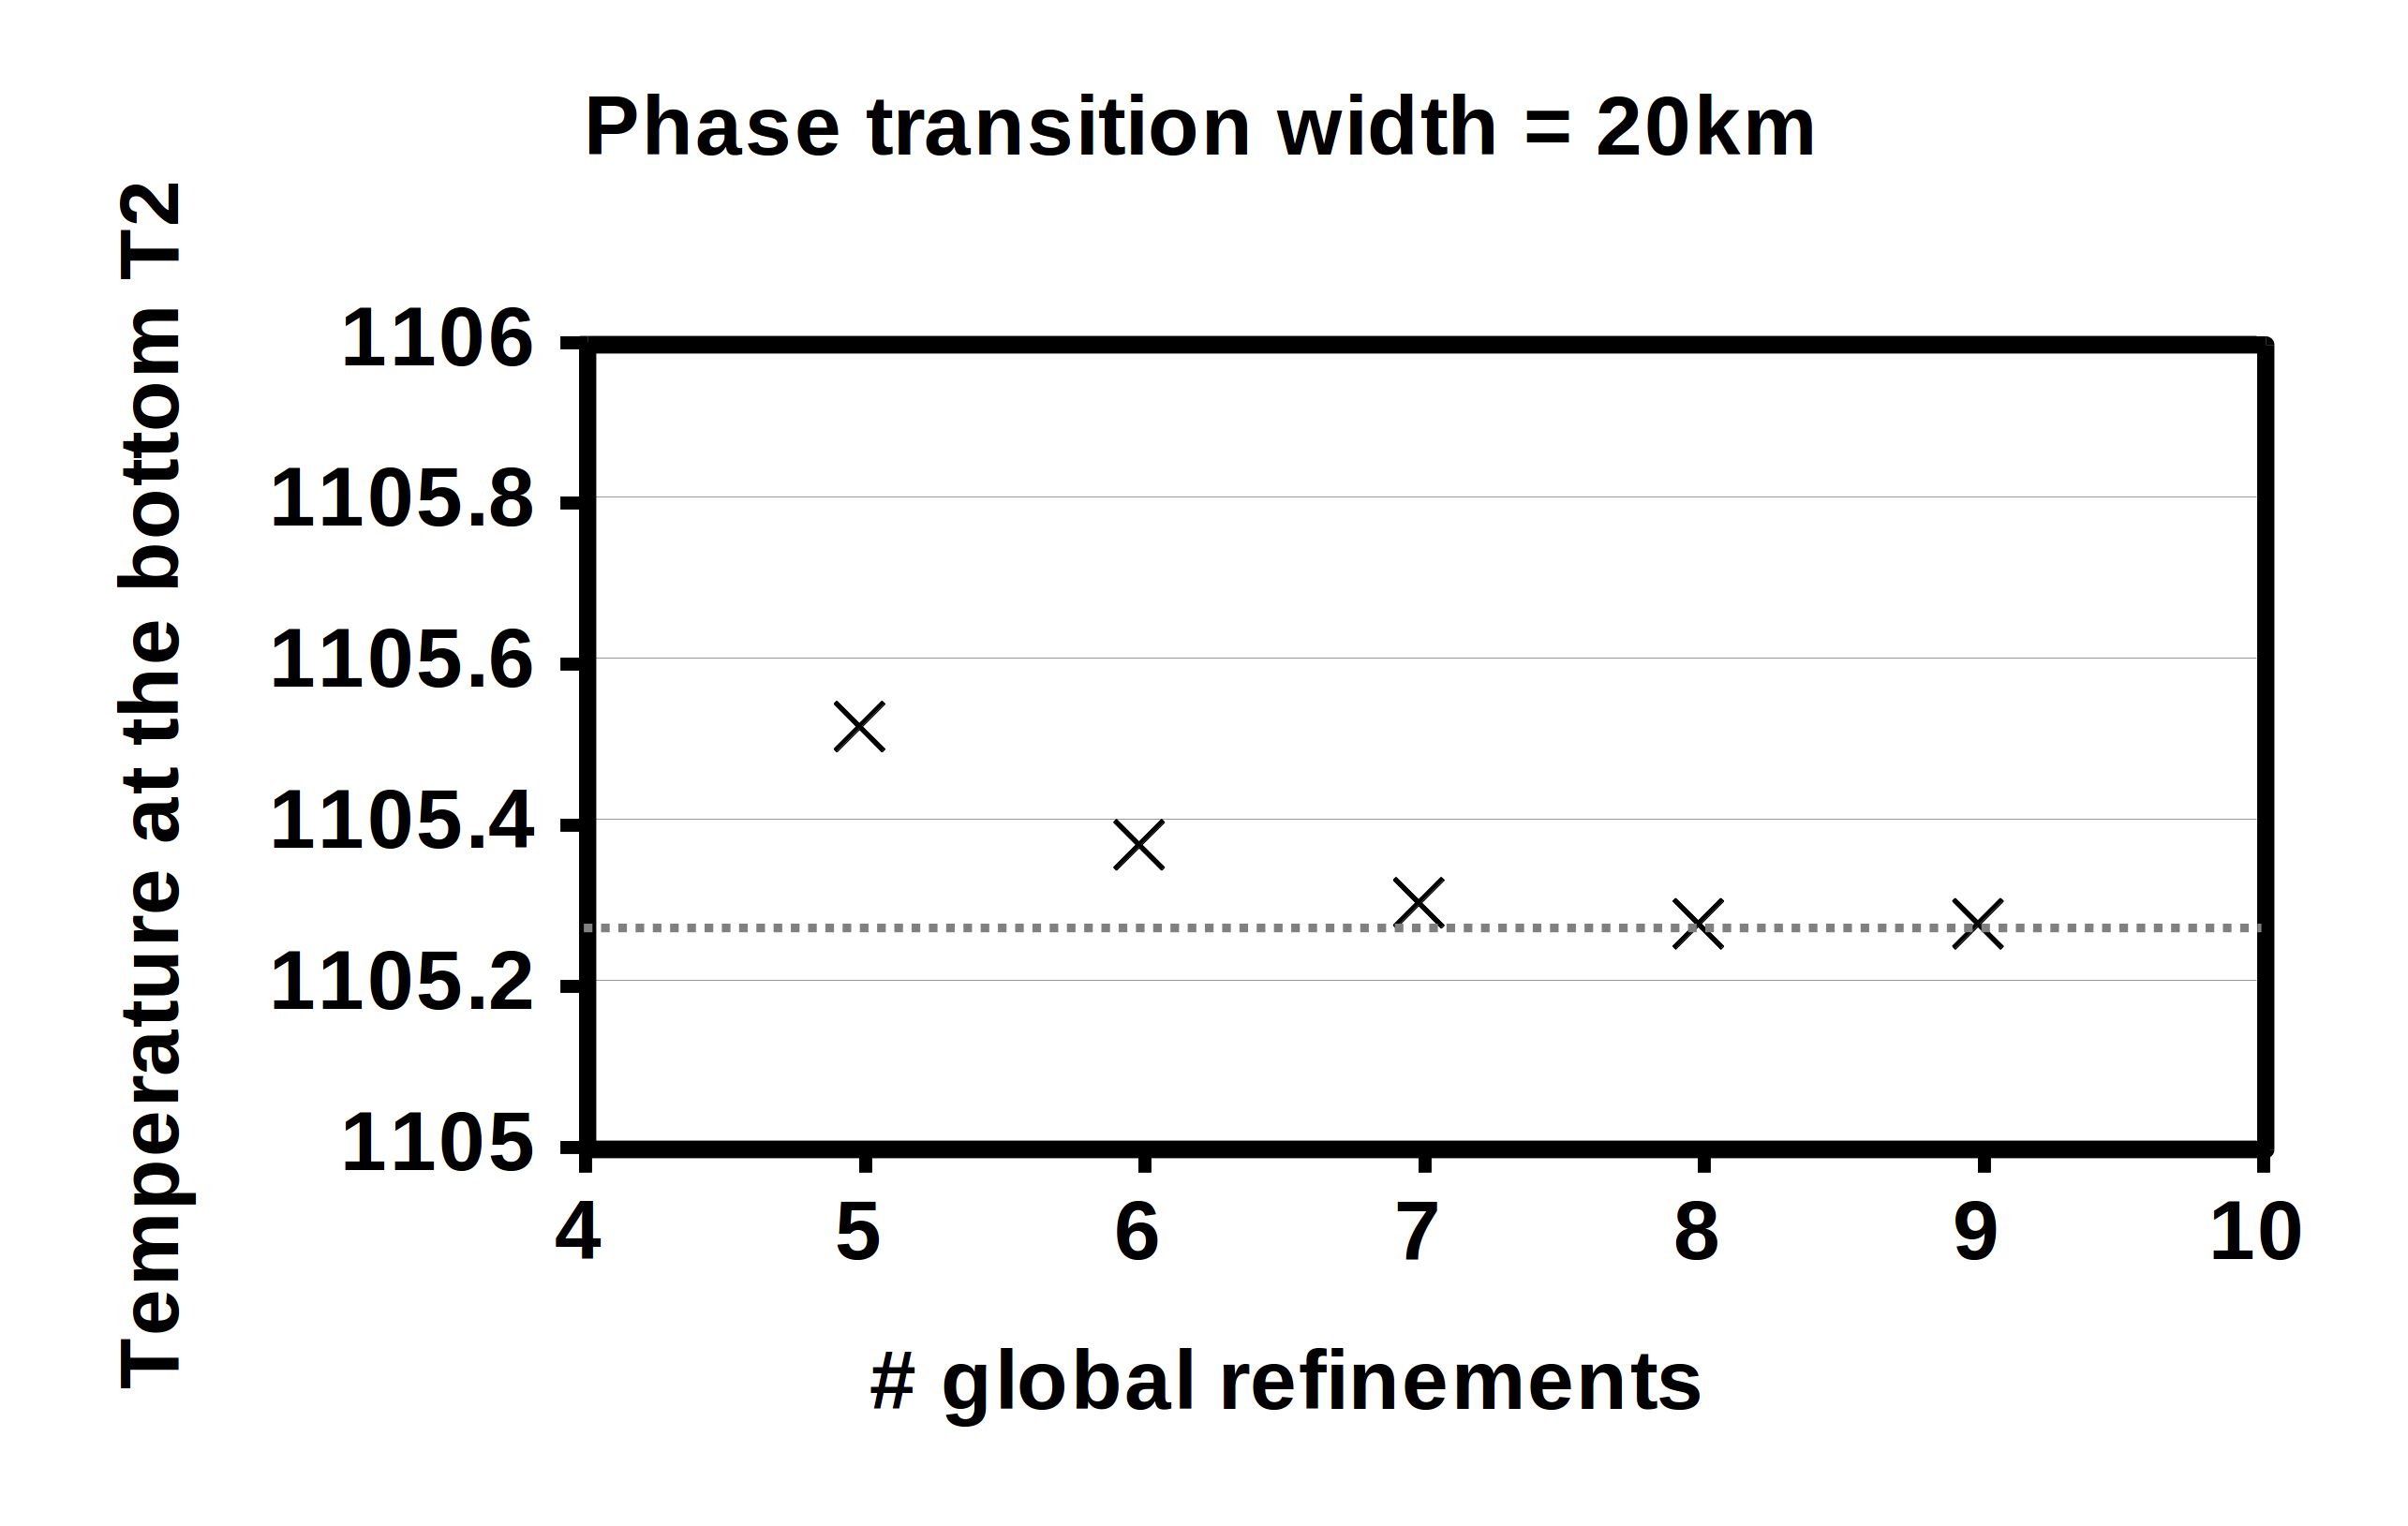
\includegraphics[width=0.49\textwidth]{cookbooks/benchmarks/latent-heat/doc/latent-heat-results-1.png}
    \hfill
    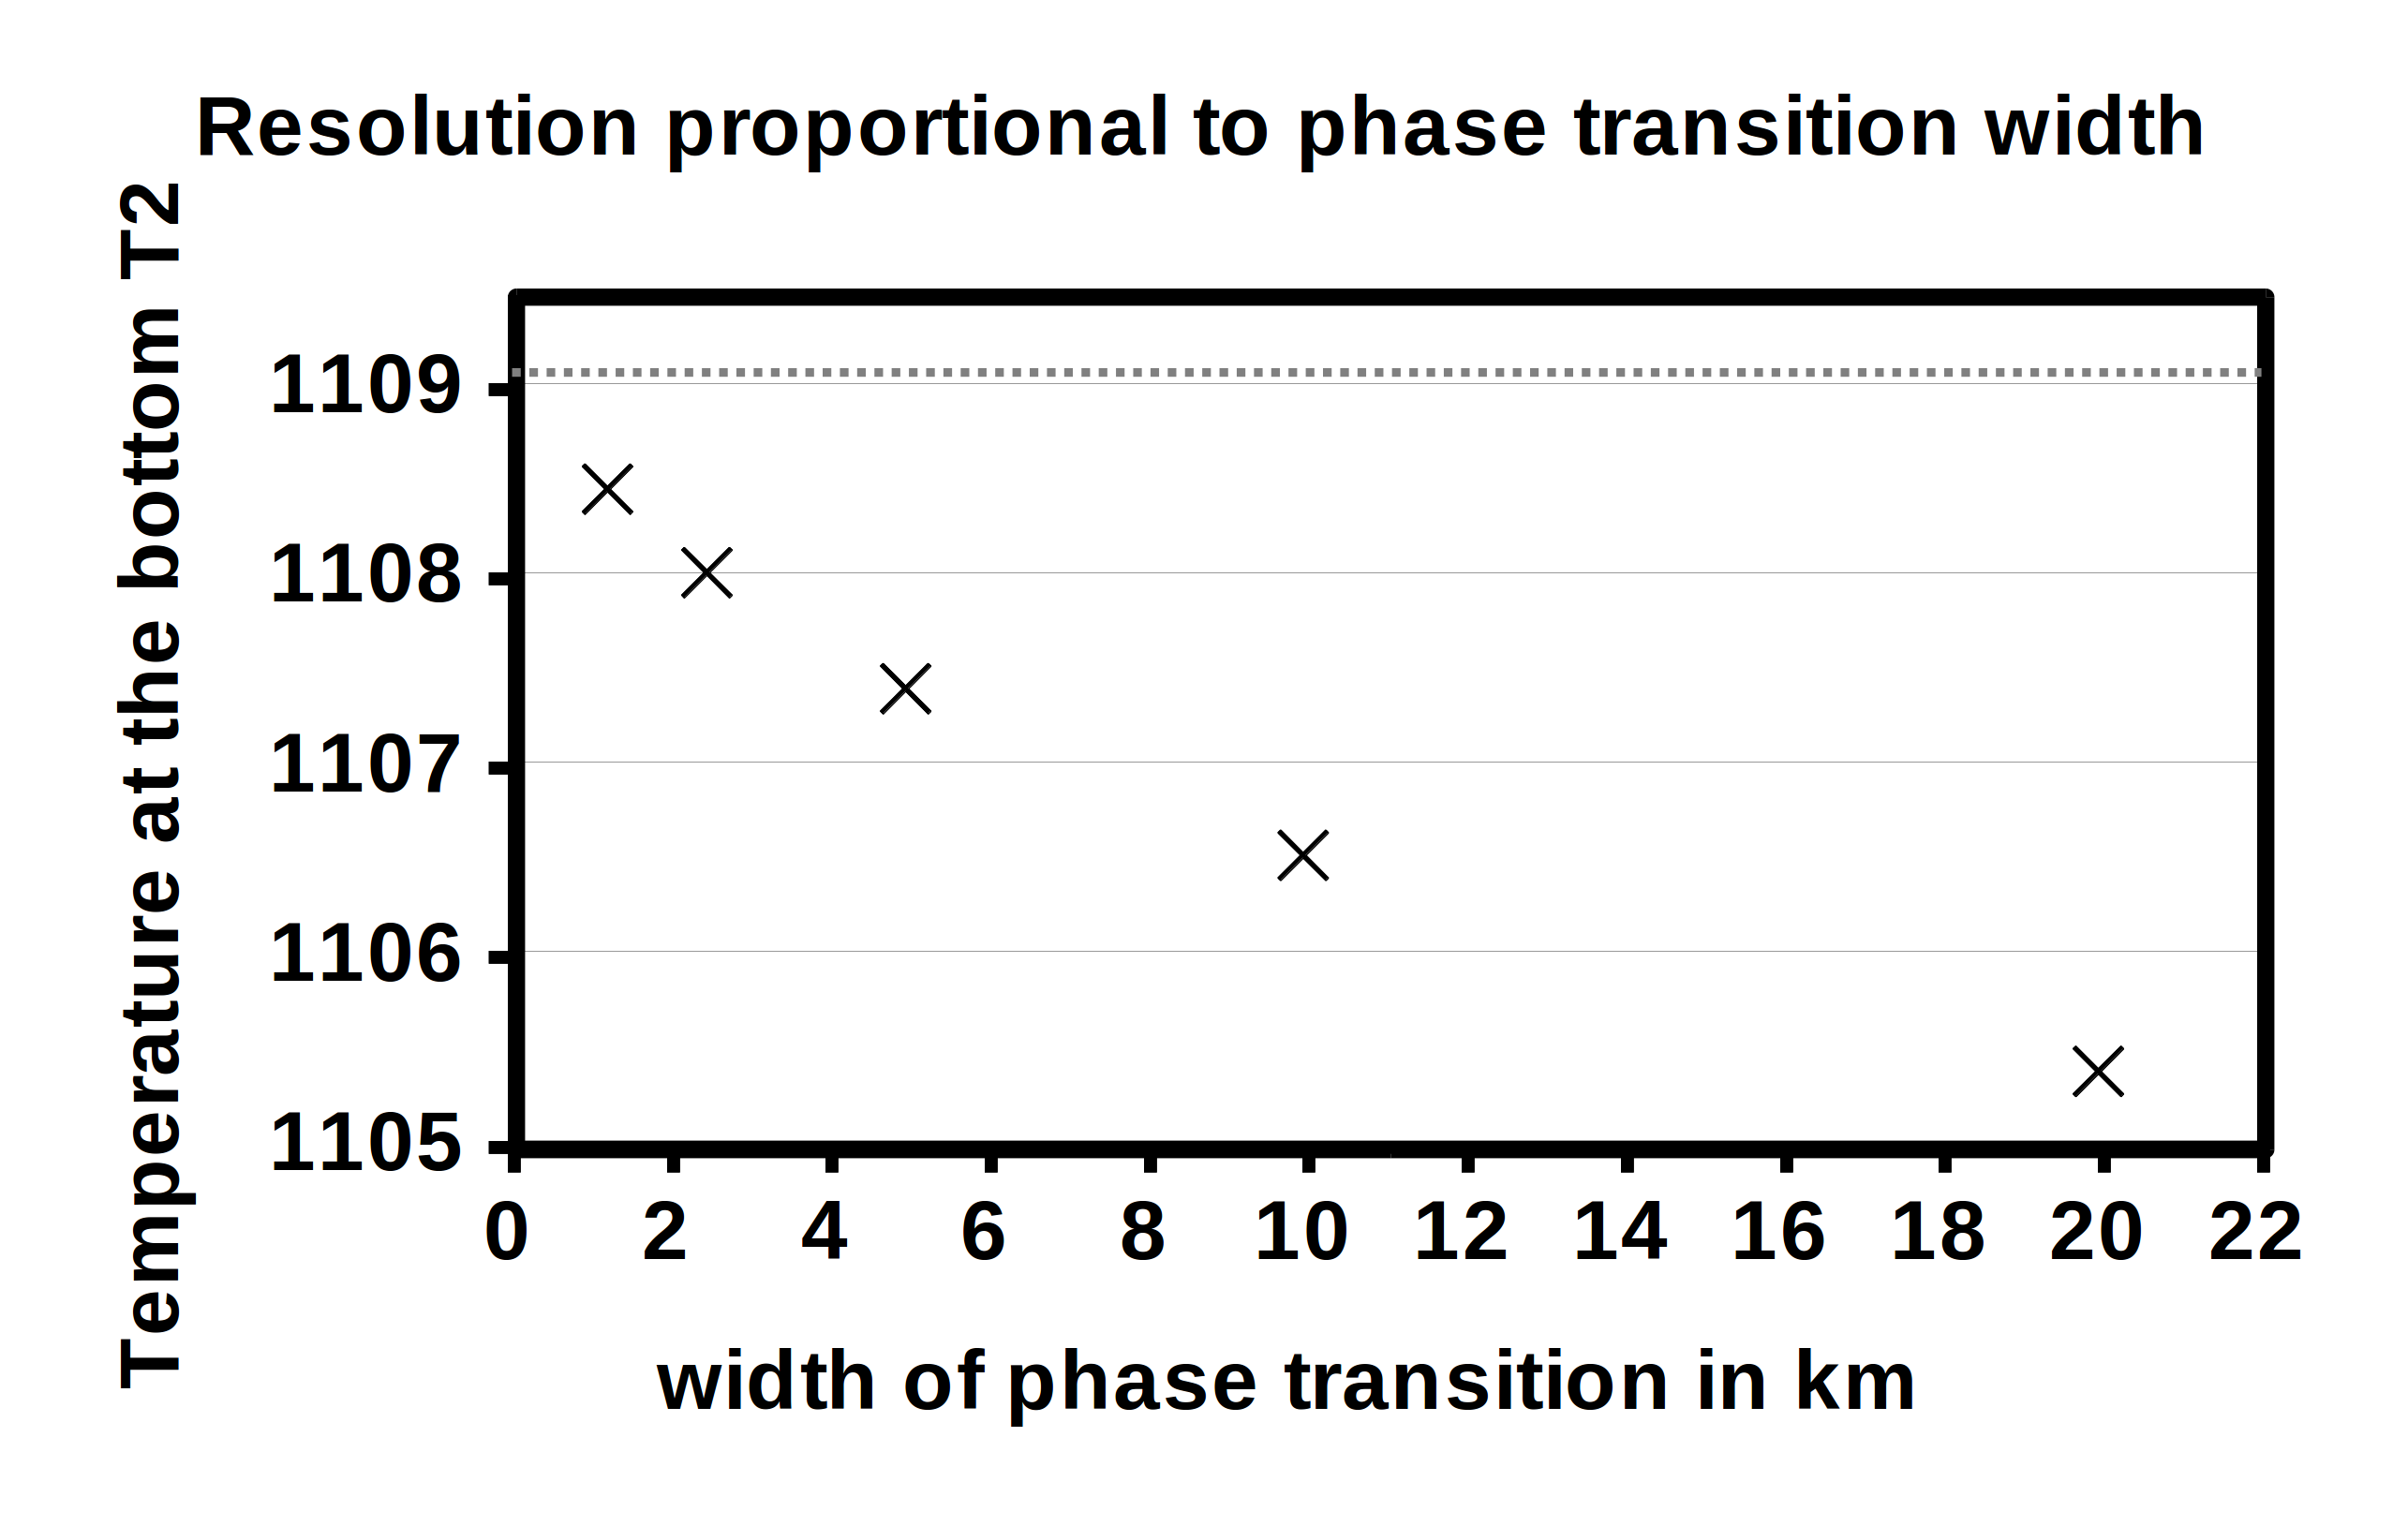
\includegraphics[width=0.49\textwidth]{cookbooks/benchmarks/latent-heat/doc/latent-heat-results-2.png}
  \end{center}
  \caption{\it Results of the latent heat benchmark. Both figures show the modelled temperature $T_2$ at the bottom of the model domain.
      Left: $T_2$ in dependence of resolution using a constant phase transition width of 20\,km. With an increasing number of global refinements of the mesh, the bottom temperature converges against a value of $T_2 = 1105.27 \, \si{K}$.
      Right: $T_2$ in dependence of phase transition width. The model resolution is chosen proportional to the phase transition width, starting with 5 global refinements for a width of 20\,km. With decreasing phase transition width, $T_2$ approaches the theoretical value of $1109.08 \, \si{K}$}
  \label{fig:latent-heat-benchmark-results}
\end{figure}

Using this input file, let us try to evaluate the results of the current
computations. We note that it takes some time for the model to reach a steady
state and only then does the bottom temperature reach the theoretical value.
Therefore, we use the last output step to compare predicted and computed values.
You can visualize the output in different ways, one of it being ParaView and shown in
Fig.~\ref{fig:latent-heat-benchmark} on the right side (an alternative is to use Visit as
described in Section~\ref{sec:viz}). In ParaView, you can plot the temperature profile
using the filter ``Plot Over Line'' (Point1: 500000,0,0; Point2:
500000,1000000,0, then go to the ``Display'' tab and select ``T'' as only
variable in the ``Line series'' section) or ``Calculator'' (as seen in
Fig.~\ref{fig:latent-heat-benchmark}). In
Fig.~\ref{fig:latent-heat-benchmark-results} (left) we can see that with
increasing resolution, the value for the bottom temperature converges to a value
of $T_2 = 1105.27 \, \si{K}$.

However, this is not what the analytic solution
predicted. The reason for this difference is the width of the phase transition
with which we smooth out the Dirac delta function that results from
differentiating the $X(y)$ we would have liked to use in an ideal world.
(In reality, however, for the Earth's mantle we also expect phase transitions
that are distributed over a certain depth range and so the smoothed out
approach may not be a bad approximation.)
Of course, the results shown above result from an the analytical approach that
is only correct if the phase transition is discontinuous and constrained to one
specific depth $y=y_{tr}$. Instead, we chose a hyperbolic
tangent as our phase function. Moreover,
Fig.~\ref{fig:latent-heat-benchmark-results} (right) illustrates what happens to
the temperature at the bottom when we vary the width of the phase transition:
The smaller the width, the closer the temperature gets to the predicted value of
$T_2 = 1109.08 \, \si{K}$, demonstrating that we converge to the correct
solution.


